\begin{center} \textbf{\huge Streaming} \end{center}
In order to deal with the continuos nature of the data, traditional programming primitives are not of much help. In order to make programmers's job easier, libraries providing higher lever abstractions are introduced. Knowing that, for a news feed classifier we need to split the 'main' stream into multiple streams to treat different portions of stream differently. For example, there needs to be at least two channels of streams branching out from the main one having the test items and training items. The main flow of the streaming logic we used is depicted in the figure.[2]\\
\begin{center}
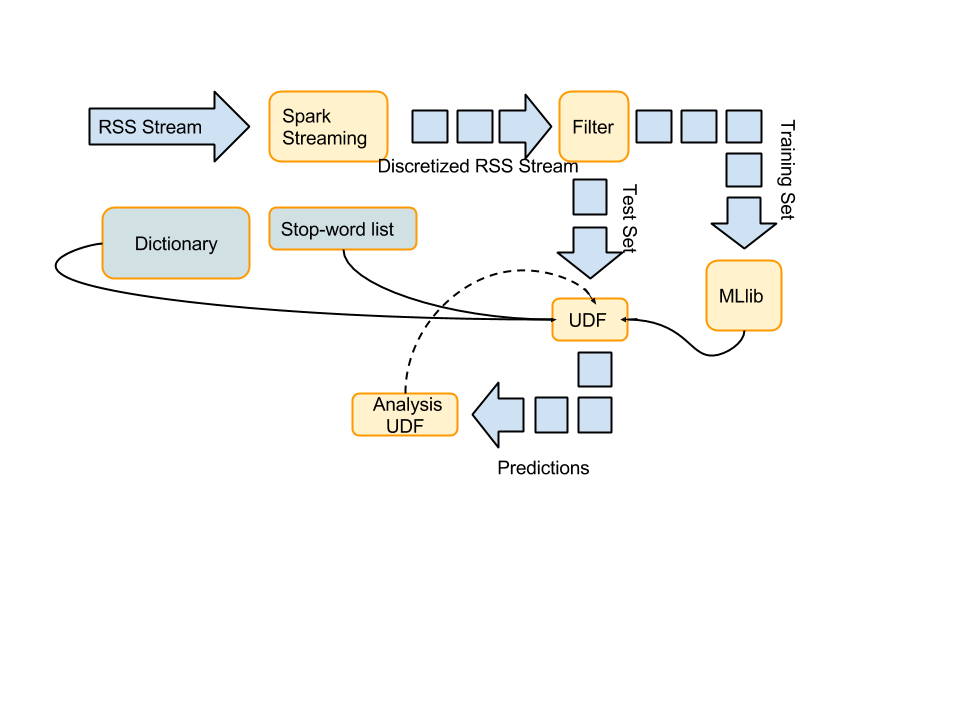
\includegraphics[width=0.2\textwidth]{./time_models/streaming_diagram}
\end{center}
